\section{Quantitative Analysis}

This section shows the analysis and discussion of our Systematic Mapping results.
We proceed by presenting bubble charts as result of combining different facets in order to 
\textit{(i)} answer the research questions and \textit{(ii)} to justify our proposal.


\subsection{Combining the facets Contribution, SLA and Data Integration Description}

\begin{figure}[h!]
\centering
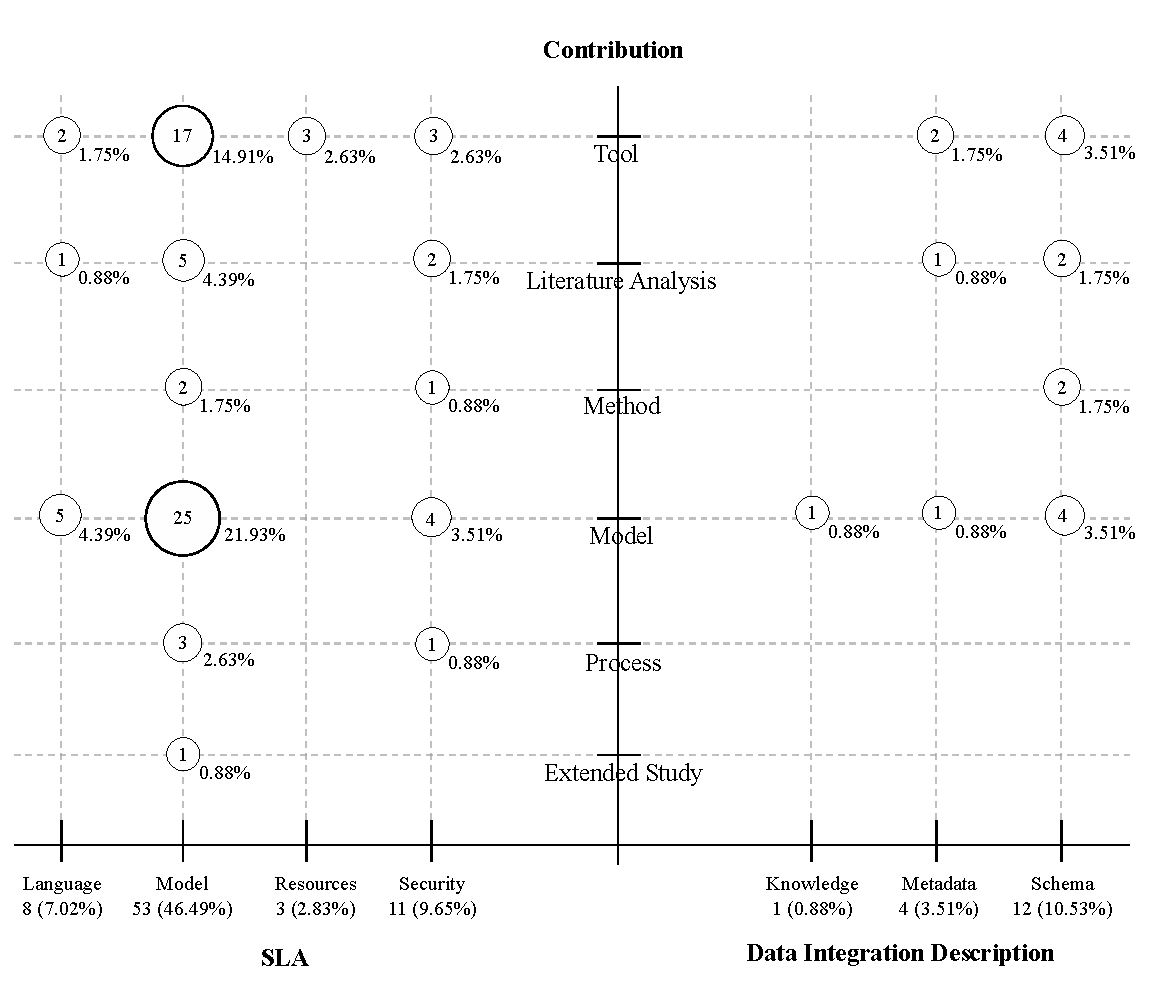
\includegraphics[scale=0.45]{figs/bubble-charts/Contribution-SLA-DIdescription.pdf} 
\caption{Contribution, SLA and Data Integration Description}\label{fig:facet1}
\end{figure}

Combining the facet Contribution with the facets SLA and Data Integration Description 
(Figure~\ref{fig:facet1}) it is possible to obtain two analysis: 
(i) how has the SLA been applied to scientific works and which are the kind of contribution 
most proposed by the authors; and (ii) which are the most applied data integration description
strategy in papers and which are the most kind of contribution associated to these works. 
Looking to the figure it is easy to note that models for SLA have been the focus in the papers 
(53 appearances - 46.49\%) followed by Security (11 appearances - 9.65\%), Language 
(8 appearances - 7.02\%) and Resources (3 appearances - 22.83\%).
Analyzing the figure is also possible to observe that Model (34 appearances - 29.82\%) and 
Tool (25 appearances - 21.93\%) are the mainly kind of contribution proposed in the papers 
followed by Literature Analysis (8 appearances - 7.02\%), Process (4 appearances - 3.51\%), 
Method (3 appearances - 2.63\%) and Extended Study (1 appearance - 0.88\%).
Regarding the data integration description, Schema (12 appearances - 10.53\%) is the most 
applied dimension followed by Metadata (4 appearances - 3.51\%) and Knowledge (1 appearance - 0.88\%).

\subsection{Combining the facets Data Integration Environment, Contribution and Research}

\begin{figure}[h]
\centering
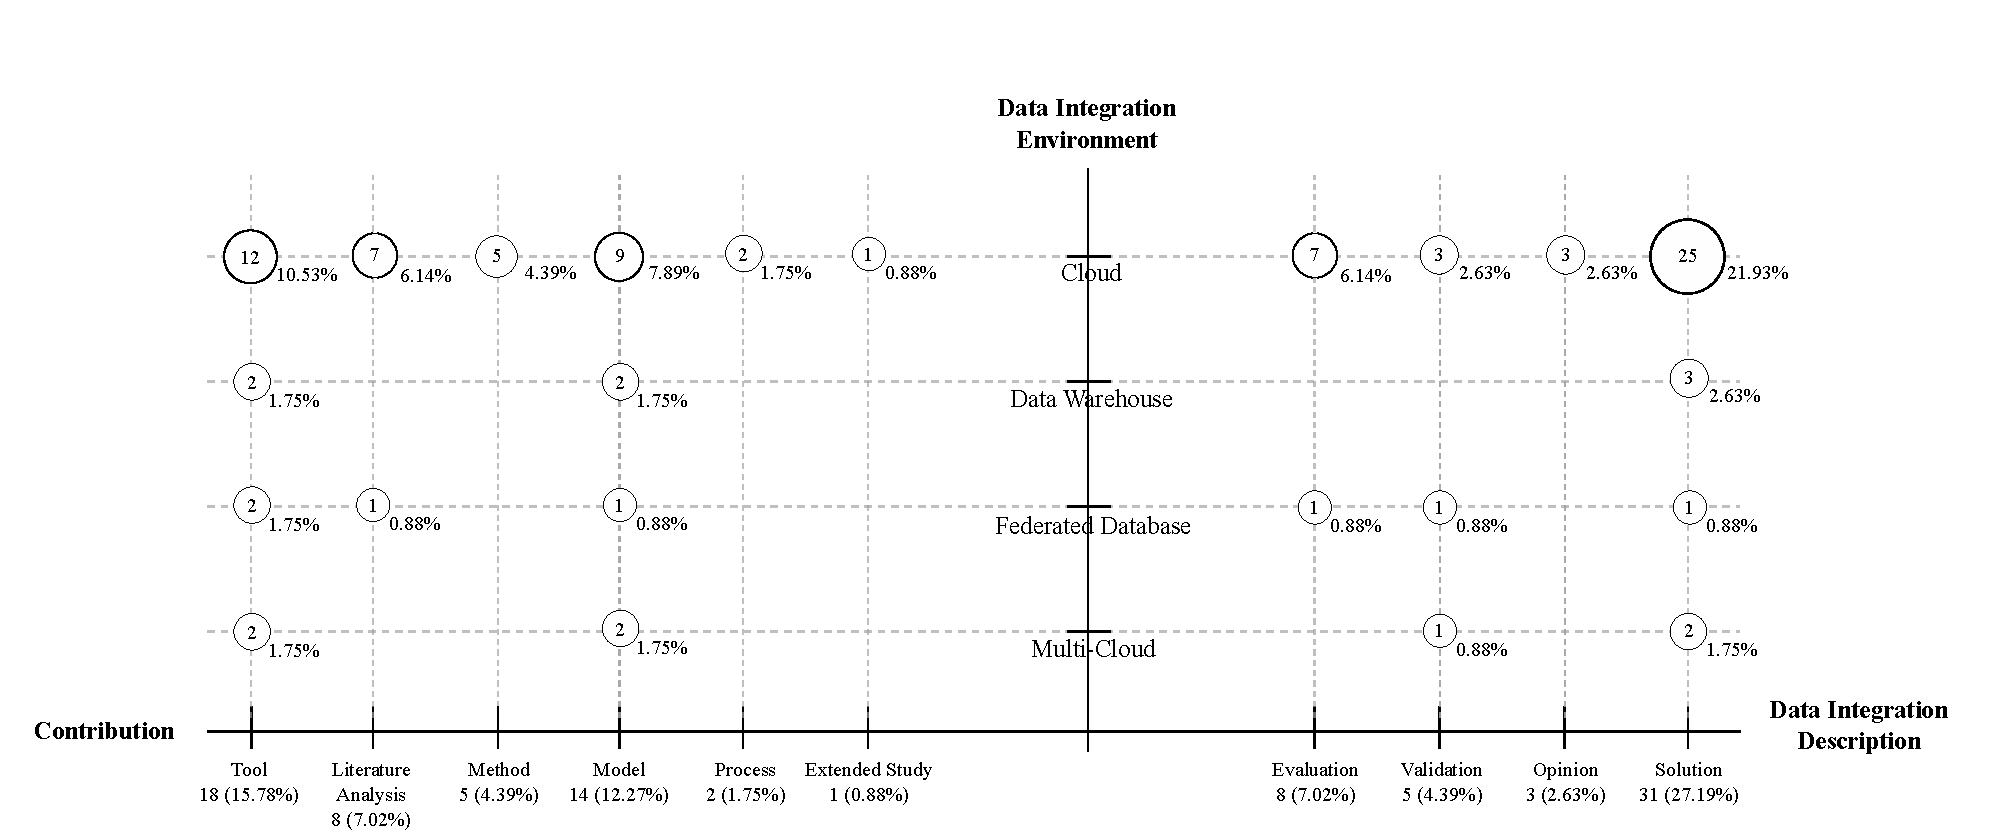
\includegraphics[scale=0.5]{figs/bubble-charts/DI-Environment-Contribution-Research.pdf}
\caption{facets Data Integration Environment, Contribution and Research}\label{fig:facet2}
\end{figure}

Combining the facet Data Integration Environment with the facets Contribution and Research 
(Figure~\ref{fig:facet2}) it is possible to observe which are the most proposed kind of
contribution and research applied to the different data integration environments.  
Looking to the figure it is easy to identify that Tool (18 appearances - 15.78\%) and 
Model (14 appearance - 12.27\%) are the mainly kind of contribution developed in the works 
followed by Literature Analysis (8 appearances - 7.02\%), Method (5 appearances - 4.39\%) 
Process (2 appearances - 1.75\%) and Extended Study (1 appearance - 0.88\%).
Analyzing the figure is also possible to observe that Solution (31 appearances - 27.19\%) is 
the type of research most developed in the papers 
followed by Evaluation (8 appearances - 7.02\%), Validation (5 appearances - 4.39\%) and
Opinion (3 appearances - 2.63\%).

\subsection{Combining the facets SLA and Contribution}

Combining the facet SLA with the facet Contribution (Figure~\ref{fig:facet3}) it is possible 
to observe how has the SLA been applied to scientific works and which are the kind of contribution 
most proposed by the authors.
Looking to the figure it is easy to note that models for SLA have been the focus in the papers 
(53 appearances).
Analyzing the figure is also possible to observe that Model (34 appearances - 29.82\%) and 
Tool (25 appearances - 21.93\%) are the mainly kind of contribution proposed in the papers 
followed by Literature Analysis (8 appearances - 7.02\%), Process (4 appearances - 3.51\%), 
Method (3 appearances - 2.63\%) and Extended Study (1 appearance - 0.88\%).

\begin{figure}[h!]
\centering
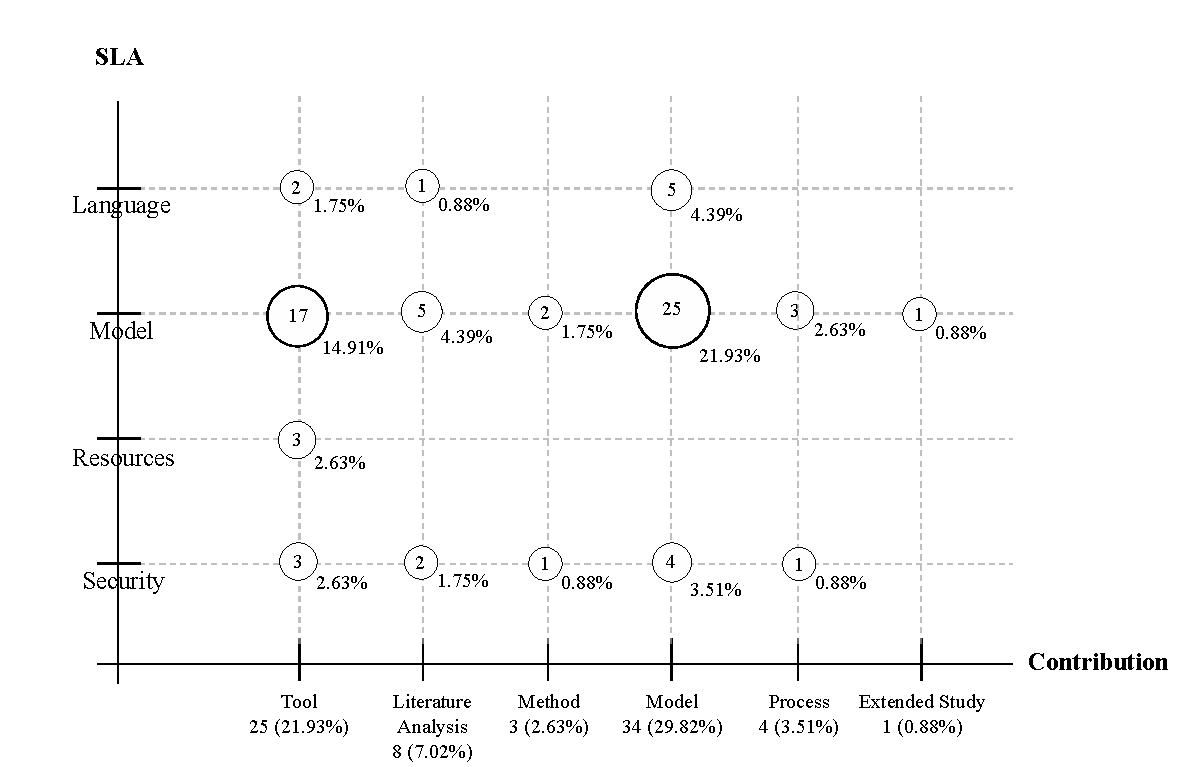
\includegraphics[scale=0.5]{figs/bubble-charts/SLA-Contribution.pdf}
\caption{Facets SLA and Contribution}\label{fig:facet3}
\end{figure}


\subsection{Combining the facets Data Quality, Data Integration Environment and Data Integration Description}

Combining the facet Data Quality with the facets Data Integration Environment e Data Integration Description
(Figure~\ref{fig:facet4}) it is possible to note which quality of service parameters have been applied most in
data integration studies.
It is also possible to identify which are the most applied data integration environment and description.
First of all, security and privacy are the most applied QoS parameter (5 appearance - 4.39\%)
followed by the other dimensions (1 appearance - 0.88\%). 
The figure also shows that SLA has not been widely used in order to address data integration solutions
(1 appearance) which reinforces our main objective of integrate SLA, data integration and multi-cloud 
environments. 
Analyzing the figure is also possible to observe that the most deployed data integration environment is 
the cloud (9.68\%) followed by multi-cloud (4.39\%), federated databases (1.75\%) and data warehouse (0.00\%).
The data integration description dimensions had the same percentage for schema, knowledge and metadata (2 appearance - 1.75\%)

\begin{figure}[h!]
\centering
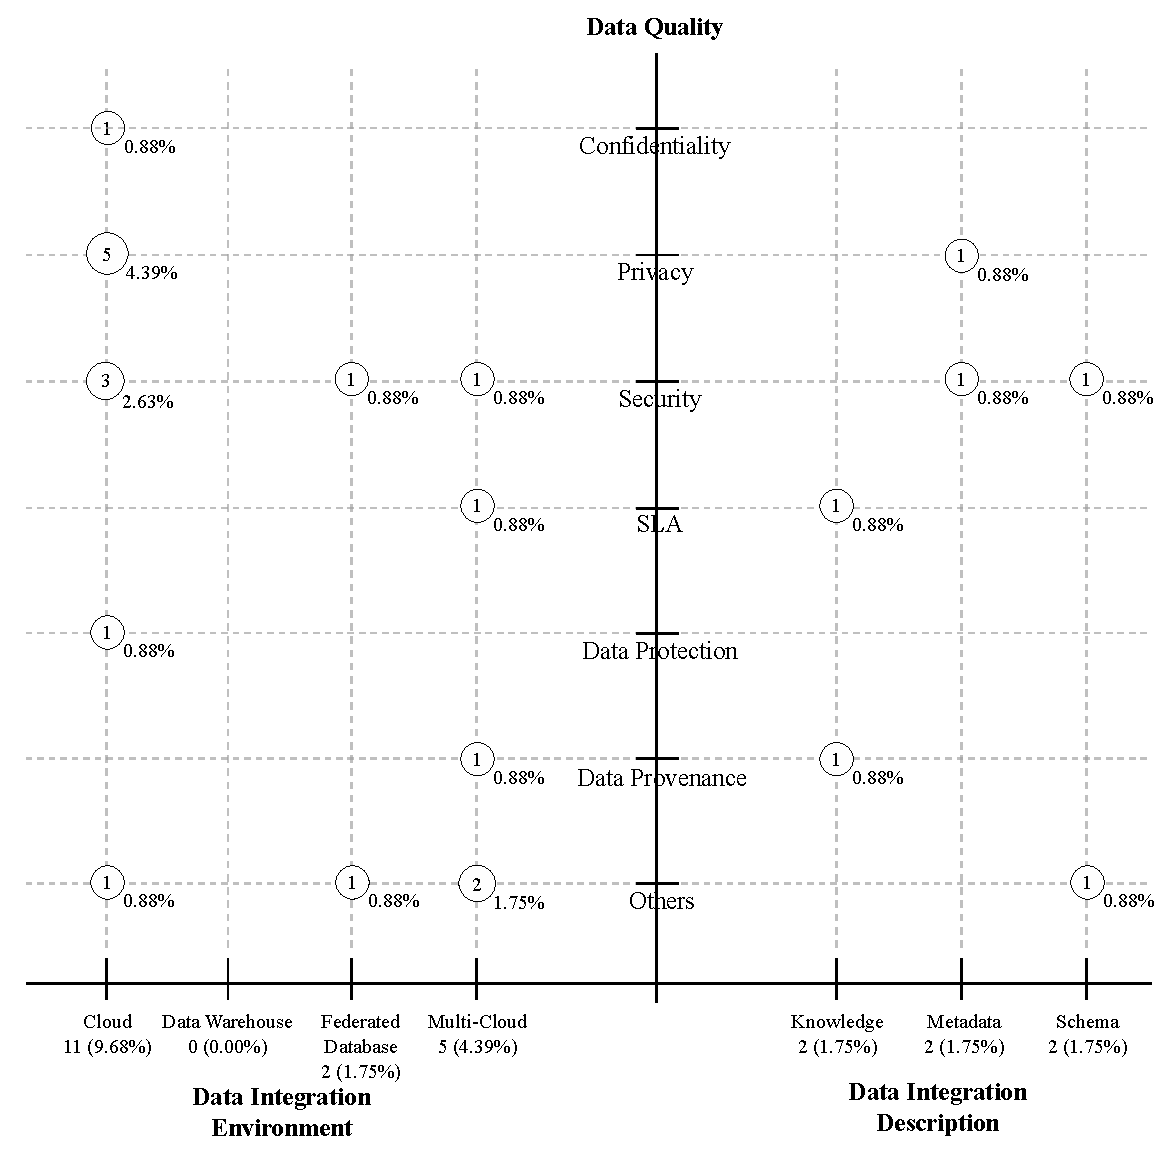
\includegraphics[scale=0.53]{figs/bubble-charts/Data-Quality-DI.pdf}
\caption{Facets Data Quality, Data Integration Environment and Data Integration Description}\label{fig:facet4}
\end{figure}
